\section{Motivation}
There has been some work in explain ability of object saliency when in comes to convolution neural network. Works like \sj{Cite Torralba, Object detectors emerge and works similar} have 
explored an avenue of explaining which objects affect the decision of a classifier the most using a combination of segmentation and perturbation techniques. 
Inspired by that we designed a simpler version of a pipeline to explain the importance of different objects in an urban scene. 
%\begin{figure*}[ht]
%	\centering
%	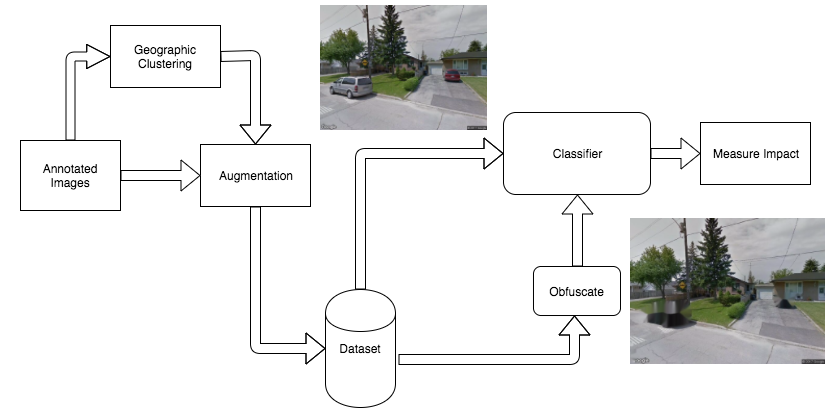
\includegraphics[width=1.4\columnwidth]{Plot/BottomupPipeline.png}
%	\caption{Process pipeline for the "Bottom Up" approach for explainability}
%	\label{fig:BUpipeline}
%\end{figure*}

The structure of this pipeline is elaborated in Fig \ref{fig:BUpipeline}. The idea is to selectively remove objects from the urban scene, and measure the change in the decision activation of the 
classifier. We start with our best performing classifier described in Section \sj{Add reference the section that describes the classifier}. To identify objects in urban scene, we use a pre-trained 
neural network called Segnet \cite{badrinarayanan2015segnet} to segment out 12 urban objects like Cars, Trees, Fences , Buildings, Pedestrians, Sidewalk, Road etc. Then we selectively in paint
\sj{Add reference for inpainting} these objects and measure the change in classification activation for beauty neuron of our classifier. These changes are directly related to the influence of that object
on the "Beauty" of that particular scene. 

%\begin{figure}[ht]
%	\centering
%	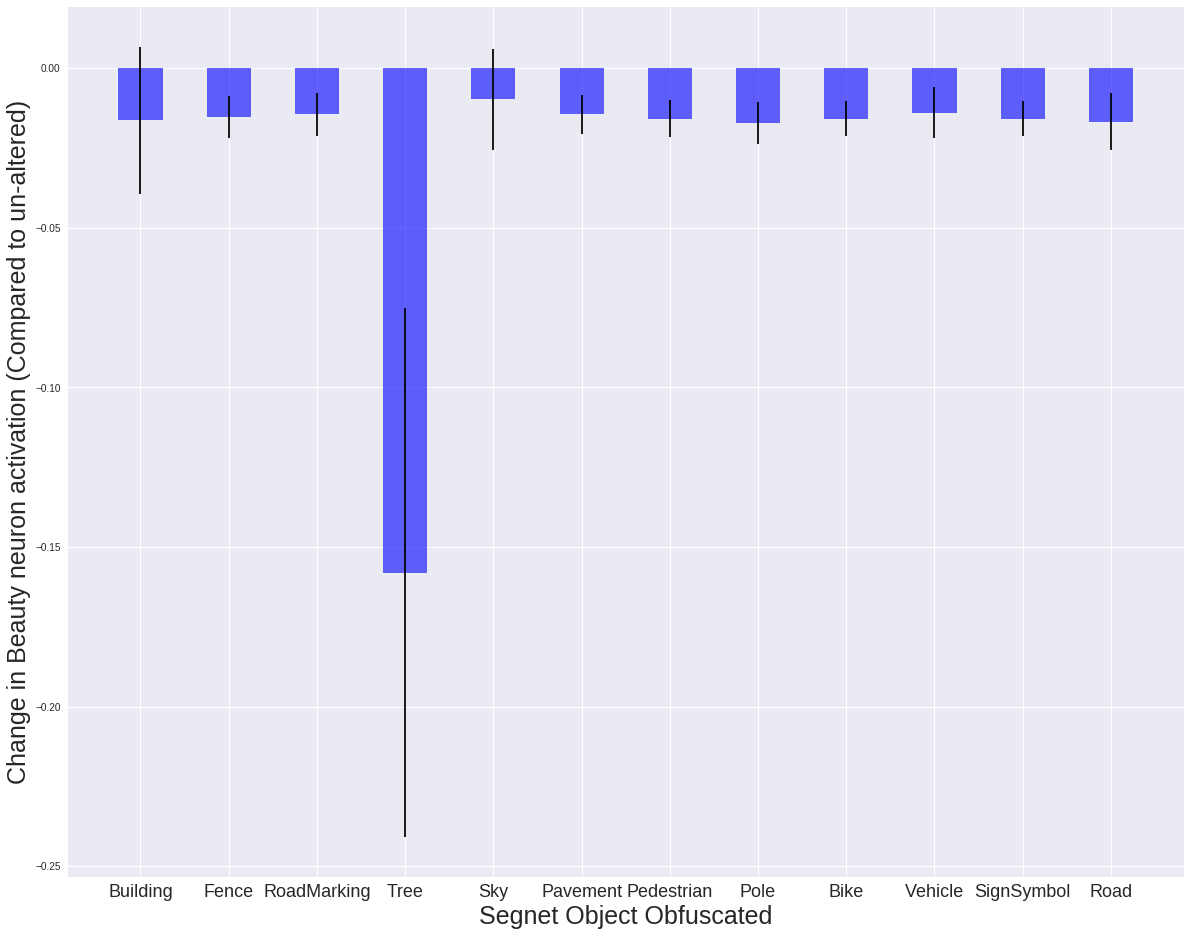
\includegraphics[width=\columnwidth]{Plot/Change_beauty_act_BottomUP.png}
%	\caption{Process pipeline for the "Bottom Up" approach for explainability}
%	\label{fig:BUActChange}
%\end{figure}

The changes in activation with the standard deviations across a random sample of 1000 images is shown in Fig \ref{fig:BUActChange}. These 1000 images were previously classified by the 
classifier as beautiful with a very high activation value. We measure the activation value of the beauty neuron after the inpainting of each object and find the difference between original beauty
activation and the perturbed activation. It is evident from the changes, that trees play a major role in deciding the beauty of a scene for the classifier. Further more we can also conjecture that Buildings and Sky, affect the beauty of an urban place in a highly variable manner. Beyond that, this method falls short in explaining in detail how the composition of an urban scene affects its beauty.
This shortcoming motivates our need to design a transformative pipeline, which not only explains importance of objects but also gives insights into compositional and design related metrics of 
a urban scene.